\documentclass[twocolumn,10pt]{article}

\usepackage[top=2cm,bottom=2cm,left=1.5cm,right=1.5cm]{geometry}


\usepackage{titlesec}
\titleformat{\section}[block]{\Large\bfseries\filcenter}{}{0pt}{}{}
% \titleformat{\subsection}[block]{\large\bfseries\filcenter}{}{}{}

\usepackage[dvipsnames]{xcolor}
\usepackage[
    colorlinks=true,
    allcolors=blue % Feel free to change the colour if you prefer another :)
]{hyperref}
\usepackage[
    backend=biber,
    style=numeric-comp,
    sortcites=true,
    giveninits=true,
    hyperref=true,
    sorting=nyt,
    natbib=true,
]{biblatex}
\addbibresource{references.bib}
\renewcommand*{\bibfont}{\footnotesize}
% Get the citations as superscipts (it's like wikipedia!?)
% thanks https://tex.stackexchange.com/questions/114987/
\DeclareCiteCommand{\supercite}[\mkbibsuperscript]
  {\usebibmacro{cite:init}%
   \let\multicitedelim=\supercitedelim
   \iffieldundef{prenote}
     {}
     {\BibliographyWarning{Ignoring prenote argument}}%
   \iffieldundef{postnote}
     {}
     {\BibliographyWarning{Ignoring postnote argument}}%
  \bibopenbracket}%
  {\usebibmacro{citeindex}%
   \usebibmacro{cite:comp}}
  {}
  {\usebibmacro{cite:dump}\bibclosebracket}
 
% thanks https://tex.stackexchange.com/a/5255 
\usepackage{amsmath}
\DeclareMathOperator*{\argmax}{arg\,max}
\DeclareMathOperator*{\argmin}{arg\,min}
\usepackage{mathtools}

\usepackage{booktabs}
\usepackage{enumitem}
\usepackage[font=footnotesize]{caption}

\usepackage{algpseudocode}
\usepackage{algorithmicx}
\usepackage{algorithm}

% \allowdisplaybreaks

\title{COMP90051 Statistical Machine Learning Project 1 Report}
\author{
Alice Johnson,
Marvin Lai,
Matthew Farrugia-Roberts}
\date{Semester 2, 2019}



\begin{document}

\maketitle


\section{Introduction}
For our class project we develop a system for automated 
authorship attribution of Twitter messages (`tweets'). We
are given a dataset of 328,932 tweets of known authorship,
and 35,437 anonymous tweets to be attributed to one of
9,297 authors as part of a class Kaggle competition.\footnote{
\url{https://www.kaggle.com/c/whodunnit},
ranking 3\textsuperscript{rd} of 162 teams
in public and private evaluation
(team name {\tt the\_shrunken\_stardust}).}

% Outline the two prevailing frameworks
Existing work on tweet authorship attribution\supercite{rocha2016authorship, bhargava2013stylometric, schwartz2013authorship}
frames the problem as either
(1) supervised multi-class classification, training models on
labelled (known-author) tweets to predict the label (author)
of test tweets, or
(2) an author profiling task, collating all tweets from an
author into a single profile and attributing each anonymous
tweet by finding the closest profile under some distance metric.
% And the two prevailing feature classes
Moreover, two broad classes of features are established as
effective:
`Static' features are hand-crafted features capturing various
stylometric aspects of writing; and
`dynamic' features are lower level patterns automatically
determined from data.

% EXPLAIN WHY WE CHOSE OUR FEATURES
Dynamic features are ideal for their simplicity and for their
robustness to our informal, non-standard and multi-lingual
text. We explore various dynamic feature classes including
byte, character, word, and flexible pattern $n$-grams.

% THEN DISCUSS OUR CHOICE OF MODELS: PROFILE-BASED OVER
% TRADITIONAL CLASSIFIERS
% Shut down traditional classification approach:
Our dataset is unique in having an extremely large number
of authors with few training tweets per author:
Over 90\% of our authors have fewer than 50 tweets,
and these tweets make up over 70\% of the dataset.
50 is the fewest tweets-per-author explored in
existing work (to our knowledge).
Multi-class classification algorithms may struggle to
generalise after seeing so few examples for most classes.

% Hit 'em with one of these profile-based method sales pitches
After seeing initially promising results from a profile-based
baseline,
we elect to focus on deeply exploring profile-based
methods, in the hope that these will scale more capably to our
`extreme' dataset.
We explore a wide range of profile-based models from recent
literature.
Furthermore, we reformulate existing distance metrics
to make them computationally tractable on our large dataset,
and we introduce a new distance metric of our own design.
% yielding improved performance over existing models.



\section{Feature classes}
We explore the appropriateness of various dynamic feature
classes for our authorship attribution task, including
character, byte, and word $n$-grams, for $n = 2,3,4,5,6$.

We also explore \emph{flexible pattern} $n$-grams, dynamic
feature classes capturing stylometric information such as
patterns in function-word use not captured by regular word 
$n$-grams\supercite{schwartz2013authorship}.
Flexible patterns are word $n$-grams where words appearing
above a certain frequency in the corpus (`high-frequency words',
or HFWs) are retained, but words appearing below a certain
frequency (`content words', CWs) are conflated. A flexible
pattern $n$-gram is a sequence of $n$ HFWs, each separated
by zero or more CWs.

% old version (did I get all of the important points above?):
% \paragraph{Flexible Patterns} Words are classified as high
% frequency words (HFWs) and/or content words (CWs) based on
% how frequently they appear in the training data. A flexible
% pattern is a sequence of HFWs separated by zero or more CWs\supercite{schwartz2013authorship}.
% We generate the $n$-grams of flexible patterns where CWs
% are replaced by tokens. This captures a pattern such ``the
% $CW$ in the'', which would not have been captured if using
% word $n$-grams\supercite{schwartz2013authorship}.

% \paragraph{Pre-processing}
We optionally \emph{pre-process} tweets,
tokenising at word and punctuation boundaries and
normalising infrequent tokens (e.g.~dates, times)
before extracting $n$-gram features.
We compare this with extracting $n$-grams directly from
raw text.


\section{Learners}

We explore several profile-based models for authorship attribution.
Each model defines an author  `profile', and a distance metric $d$
between these profiles and new tweets.
We learn profiles for a set $\mathcal{A}$ of candidate authors from
a corpus of tweets, and then predict the author of each new tweet
$t$ as $\argmin_{a \in \mathcal{A}} d(a, t)$.
% \footnote{For CNG, we additionally handle ties
% by selecting the author with the most tweets in the corpus.}
The models are as follows.

\paragraph{Common N-Gram (CNG)}
\hypertarget{par:cng}{}
The CNG model\supercite{kevselj2003n} defines an author's profile
as the normalised frequencies of the $L$ most common $n$-grams
across all of the author's tweets, where $L$ is a hyper-parameter.
$d_{cng}$ measures distance between author $a$ and tweet $t$ as
$$
d_{cng}(a, t) =
    \smashoperator{\sum_{x \in X_a \cup X_t}}\ 
        {\left ( \frac{2 \cdot (P_a(x) - P_t(x))}{P_a(x) + P_t(x)} \right )}^2
$$
where
$X_a$ is the set of $n$-grams in author $a$'s profile
(i.e.~their $L$ most frequent $n$-grams),
$X_t$ is the set of $n$-grams in $t$,
$P_a(x)$ is the normalised frequency of $n$-gram $x$ in $a$'s
tweets (or 0 if $x \notin X_a$),
and
$P_t(x)$ is $x$'s normalised frequency in $t$.

This sum over all $n$-grams in $X_a \cup X_t$ is expensive
to compute for every author, for every test tweet.
We exploit the sparsity of our $n$-gram features by using
an equivalent\footnotemark~formulation in terms of a sum over
only $X_a \cap X_t$:
$$
d_{cng} (a, t) =
    \smashoperator{\sum_{x \in X_a \cap X_t}}\ 
        {\left ( \frac{2 \cdot (P_a(x) - P_t(x))}{P_a(x) + P_t(x)} \right )}^2
        - 8 \cdot |X_a \cap X_t| + C
$$
where $C=4 \cdot (L + |X_t|)$ is a constant.
We can efficiently compute this sum (and $|X_a \cap X_t|$)
using an inverted index.
\footnotetext{See notes on reformulating CNG in appendix \hyperref[A1]{A.1}.}

\paragraph{Source Code Author Profile (SCAP)}
In SCAP\supercite{frantzeskou2006effective} an author's profile
comprises the set of the $L$ most common $n$-grams across the
author's tweets. $d_{scap}$ is then defined in terms of the
overlap of this set with that of the test tweet:
$$
% display fraction (looks much nicer)
% d_{scap}(a, t) = 1 - \frac{|X_a \cap X_t|}{L}
% inline fraction (if space needed)
d_{scap}(a, t) = 1 - |X_a \cap X_t| / L
$$

As $d_{scap}$ is already in terms of only $X_a \cap X_t$, we can
efficiently compute it for many authors using an inverted index.

\paragraph{Recentered Local Profile (RLP)}
\hypertarget{par:rlp}{}
RLP\supercite{layton2012recentred} builds profiles
from the $L$ $n$-grams with the highest absolute `recentered'
normalised frequency,
$RP_a(x) = P_a(x) - E(x)$
where $P_a(x)$ is the normalised frequency of $n$-gram $x$ in
$a$'s tweets, and
$E(x)$ is the normalised frequency of $x$ in all tweets.
%\footnote{Conceptually, $E(x)$ approximates the probability
%distribution of $n$-grams over the English language. As the
%probability distribution of $n$-grams over the English language
%is unknown, and the data set is not exclusively in English, we
%approximate $E(x)$ by calculating the normalised frequencies
%of all $n$-grams in the training set.}
Defining $RP_t(x)$ similarly, 
$d_{rlp}$ is a cosine distance over
$X_a \cup X_t$:\footnote{
This is a corrected version of the formulation in \cite{layton2012recentred},
based on \cite{layton2014tutorial}.}
$$
d_{rlp}(a, t) = 1 -
\frac{\displaystyle
    \smashoperator{\sum_{x \in X_a \cup X_t}}
        RP_a(x) \cdot RP_t(x)
}{\displaystyle
    \sqrt{\smashoperator[r]{\sum_{x \in X_a \cup X_t}} RP_a(x)^2
    \cdot \smashoperator{\sum_{x \in X_a \cup X_t}} RP_t(x)^2}
}
$$

As with CNG, this calculation is prohibitively expensive at our scale.
An exact formulation in terms of only $X_a \cap X_t$ is not possible,
so we approXimate RLP (XRLP) instead\footnotemark:
\footnotetext{See derivation of XRLP in appendix \hyperref[A2]{A.2},
including addendum.}
$$
d_{xrlp}(a, t) = 1 -
\frac{\displaystyle
    \smashoperator[r]{\sum_{x \in X_a \cap X_t}}
        RP_a(x) \cdot P_t(x)
    - \smashoperator{\sum_{x \in X_a}}
        RP_a(x) \cdot E(x)
}{\displaystyle
    \sqrt{\smashoperator[r]{\sum_{x \in X_a}} RP_a(x)^2
    \cdot \smashoperator{\sum_{x \in X_t}} RP_t(x)^2}
}
$$
The sum over $X_a \cap X_t$ can be computed using an inverted index,
the sums over $X_a$ are independent of $t$ and can thus be pre-computed,
and the sum over $X_t$ is a constant.

% % \paragraph{Simplified RLP (SRLP)}
% We also adapt the RLP method further by proposing an
% additional, simplified, efficiently computable distance metric
% based on the same profiles---Simplified RLP (SRLP):
% $$
% d_{srlp}(a, t) =
%     \smashoperator[l]{\sum_{x \in X_a \cap X_t}}
%         \frac{ RP_a(x) } { |RP_a(x)| }
%         \cdot
%         \frac{ RP_t(x) }{ |RP_t(x) | }
% $$

\paragraph{Smooth $P_a$ Cross Entropy (SPaCE)}
\hypertarget{par:space}{}
We present a new model for profile-based authorship attribution.
SPaCE defines a profile using the \emph{smoothed} normalised
$n$-gram frequencies from the author's tweets, including for
unseen $n$-grams. 
We interpret these normalised frequencies as a probability
distribution over the set of all $n$-grams, and use the cross
entropy between the probability distributions of $t$ and $a$
(plus a per-author offset capturing author prolificacy)
as our distance metric:
$$
d_{space}(a, t) =
    - \ln (P(a)) / N_t
    - \sum_{x \in X_t} P_t(x) \ln (P'_a(x))
$$
$P(a)$ is the proportion of corpus tweets by $a$,
$N_t$ is the total number of $n$-grams in $t$, and
$P'_a(x)$ is the smoothed probability of $x$.
$P'_a(x)$ is defined in terms of $P_a(x)$ using either
(i)   add-$k$ smoothing;
(ii)  linear interpolation with $E(x)$ by $\alpha$; or
(iii) linear interpolation with $E(x)$ by $\exp(-N_a/K)$,
      an amount decaying exponentially with $N_a$,
      the total number of $n$-grams in $a$'s tweets.
$K$, $\alpha$, and $k$ are hyper-parameters.

While smoothing destroys the sparsity of profiles, it's still
possible to efficiently compute $d_{space}$ for many authors.\footnotemark
\footnotetext{See notes on computing SPaCE in appendix \hyperref[A3]{A.3}.}

\paragraph{Ensemble}
We create a simple ensemble in an attempt to combine multiple
dynamic feature classes in a single model.
We use SCAP as a base learner for its computational simplicity,
and attribute tweets to the author selected by the most
base models (i.e. by unweighted relative majority vote).




\section{Experiments}
In this section, we detail our experimental setup for tuning
and comparatively evaluating each combination of learner and dynamic feature class, and we report our results.
% Since our eventual goal is to attribute each of the unlabelled
% tweets with high accuracy, we adopt accuracy as our performance
% measure.

\paragraph{Data split}

% Aside from through the public leaderboard scores (derived from a
% small number of tweets), we can't know the true authors of the
% unlabelled tweets ahead of the competition end time. This means we
We
are unable to effectively use our unlabelled tweets to compare
the accuracy of different learner/feature class combinations,
since the public leaderboard scores are derived from a small
number of tweets.
In response, \emph{we create our own, larger validation dataset}
by randomly partitioning our labelled dataset in two, as follows:

\begin{itemize}[itemsep=0pt,topsep=0pt]
    % We can collapse this list inline if necessary for space.
    \item \textbf{Validation data}: 69,838 tweets (20\% of labelled data)
    reserved for final evaluation of each learner/feature class combination,
    to be used for final model selection.
    \item \textbf{Reduced training data}: Remaining 259,094 tweets (80\%),
    to be split further for use training and tuning each learner/feature
    class combination.
\end{itemize}


\paragraph{Feature engineering}

Across our experiments with each learner/feature class combination,
we observe
(1) character $n$-grams are most effective for $n=4,5,6$, and with raw
    text input;
(2) byte $n$-grams perform indistinguishably from character $n$-grams;
(3) word $n$-grams perform best for $n=2$, where they benefit slightly
    from our pre-processing; and
(4) flexible pattern $n$-grams perform best with $n=2,3$.
Figure~\ref{fig:features} exemplifies some of these relationships.
For brevity, we report only results from learners trained on these
high-$n$ character $n$-grams and low-$n$ word/flexible pattern $n$-grams.

\begin{figure}[h]
    \centering
    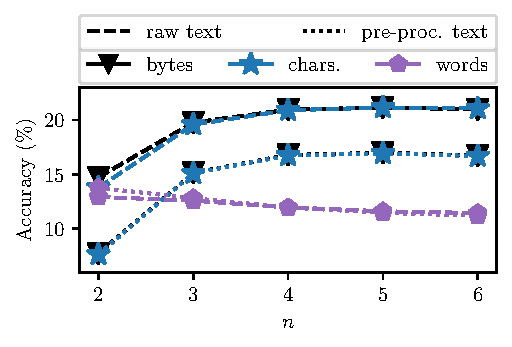
\includegraphics[
        width=\columnwidth,
        trim=0 2ex 0 1.6ex,
        clip
    ]{effect-of-n.pdf}
    \caption{Effect of pre-processing and $n$ on SCAP, fixed $L=300$.}
    \label{fig:features}
\end{figure}

\vspace{-3ex}
\paragraph{Hyper-parameter tuning}

For each learner/feature class combination, we tune our hyper-parameter
using grid search optimisation on the reduced training data, as follows:

We tune the profile length $L$ for SCAP using an 8-fold cross-validated
grid search over the reduced training data.

Evaluating each configuration of CNG, and XRLP is more
computationally expensive, so for these models we tune $L$ using
holdout validation rather than 8-fold cross validation
(we train on 87.5\% of the reduced training data, and select the $L$
giving the highest accuracy on the other 12.5\%).

SPaCE models are our most computationally expensive to evaluate,
since smoothing removes the sparsity of profiles.
To tune the hyper-parameter for each smoothing method
($k$ for method i, $\alpha$ for method ii, and $K$ for method iii)
we perform a grid search using holdout validation on the reduced training
data, evaluating on 1000 tweets (0.3\%).
Due to time constraints, we only tune on character $n$-grams.

For our ensemble, we try various combinations of features, and use
holdout validation to select the best combination
(seven SCAP base models using character 2--6-grams, word 2-grams,
and flexible pattern 2-grams, respectively).


\paragraph{Model selection}
After tuning each learner/feature class combination as above,
we re-train the tuned configurations on the entire reduced
training set, and measure accuracy with our validation data.
Table \ref{tab:devresults} summarises our results.

\begin{table}[h]
\centering
\begin{tabular}{@{}cccccccc@{}}
\cmidrule{3-8}
Acc. (\%)   &     & \multicolumn{6}{c}{Feature class}                    \\
\cmidrule{3-8} 
            &     & \multicolumn{3}{c}{character} & word  & \multicolumn{2}{c}{flex. patt.} \\
\cmidrule(r){1-1} \cmidrule(rl){3-5} \cmidrule(rl){6-6} \cmidrule(rl){7-8} 
Models      & $n$ & 4      & 5      & 6           & 2     & 2     & 3    \\
\cmidrule(r){1-1} \cmidrule{3-8} 
CNG         &     & 25.4   & 26.2   & 26.4        & 20.5  & 13.8  & 12.5 \\
SCAP        &     & 21.7   & 22.2   & 22.1        & 14.4  &  9.7  &  8.5 \\
XRLP%\footnotemark
            &     & 18.6   & 18.4   & 17.4        & 12.4  &  9.4  & 10.0 \\
% SRLP        &     & 23.7   & 25.4   & 25.7        & 18.3  & 12.5  & 11.9 \\
SPaCE i     &     & 27.5   & 28.3   & 28.0        & ---   & ---   & ---  \\
SPaCE ii    & &{\bf 32.7}  & 32.2   & 30.9        & ---   & ---   & ---  \\
SPaCE iii   &     & 32.5   & 31.5   & 30.1        & ---   & ---   & ---  \\
                  \cmidrule{3-8} 
Ensemble    &     & \multicolumn{6}{c}{ ---23.4--- }\\ % (char23456grams+word2grams+flex2grams)
\bottomrule
\end{tabular}
\caption{Tuned model accuracy on held-out validation data.}
\label{tab:devresults}
\end{table}
% \footnotetext{See appendix \hyperref[A2]{A.2}:
% These results are from XRLP with a small bug.}

\vspace{-2ex}
We re-train our best performing model/feature class combination
(SPaCE ii, character 4-grams) on the entire labelled dataset for
submission,
achieving a public score of \textbf{34.7\%} accuracy,
and \textbf{35.0\%} accuracy on the private dataset.

\section{Critical analysis}

% Matt: I think maybe we should LEAD this section with the
% SPaCE discussion? Since it's our strongest model.

% SPaCE is better than all profile methods. Why? - Matt
\paragraph{SPaCE}
We observe that SPaCE models outperform all other models for
character-level $n$-grams.
Minimising $d_{space}$ corresponds to maximising
tweet (log) likelihood assuming tweets are sequences of
$n$-grams drawn independently from their author's $n$-gram
probability distribution.
It's somewhat surprising to see this level of performance,
given the naivety of this assumption.
However, SPaCE uses a much richer profile representation
than other methods, with smoothing providing effective
regularisation. This may help it to make finer grained
distinctions between authors.

The choice of smoothing method is critical.
We see additive smoothing (i) outperformed by interpolation
smoothing (ii, iii).
Additive smoothing corresponds to
% "assuming a uniform prior on $n$-gram probability distributions
% when estimating profiles,"
% NO! That's subtly wrong, it's a non-uniform distribution over
% probability distributions.
MAP estimation of profiles with a prior distribution 
(over $n$-gram distributions) concentrated about the uniform
$n$-gram distribution,
while interpolation methods take corpus-level frequency
information into account.
Since authors' $n$-gram distribution are indeed highly
non-uniform, interpolation smoothing is theoretically
more appropriate.


% Compare local profile methods and compare to results found in literature - Alice
\paragraph{CNG, SCAP, XRLP} Recent works show RLP outperforms CNG
on large documents with few authors\supercite{layton2012recentred},
and SCAP outperforms CNG when there is limited training data per
author\supercite{frantzeskou2006effective}.
In contrast, we see CNG outperforming both SCAP and (X)RLP.
XRLP may be under-performing due to our small (per author)
dataset---profiles based on recentered frequencies may be unreliable
when computed from noisy $n$-gram counts.
CNG's under-performance in \cite{frantzeskou2006effective} with
profiles shorter than $L$ may be due to a flaw in the distance
metric, which our reformulation implicitly overcomes (we correct
for short profiles by using a constant offset term, effectively
assuming all authors have at least $L$ $n$-grams).

% compare character grams versus word and flex grams - Marvin
\paragraph{Features}

% characters reign supreme: character density per-tweet explains?
We see character $n$-grams enabling greater accuracy compared to word
and flexible pattern $n$-grams.
Our lack of data (per author) may be responsible;
The same amount of text from a given author yields more character $n$-grams
than word or flexible pattern $n$-grams, possibly leading to a more
discriminating learned profile.

% flex patterns v. words: trading off structure/content.
% maybe in this dataset content is more reliable.
We further observe word-based models consistently outperforming
flexible pattern-based models. Flexible pattern $n$-grams are similar to
word $n$-grams in their number of $n$-grams per tweet, but they
sacrifice content information about an author's text by retaining only HFWs,
thereby striking a different position on a style/content information
trade-off. 
While word $n$-grams are not necessarily superior in general, it seems
that content is more salient in our task.

% Combining the features in the ensemble performed better than word
% and flexible pattern by itself. Suggests ... orthogonal? - Shared
Character, word and flexible pattern $n$-grams are individually
incomplete representations of text.
Combining the features in the ensemble model must capture more
information about authorship, suggesting that our feature classes
are somewhat orthogonal.
Future work may investigate more sophisticated methods for
combining multiple dynamic feature classes into a more robust model. 


\printbibliography

\section{Appendix}

\subsection*{A.0 Inverted index computation}
\label{ax:invertedindex}

Consider computing a sum $s(A)$ of some function $f$ over the elements
in the intersection of two sets $A$ and $B$, for many $A$ in some
family $\mathcal{A}$, with each $|A| \gg |B|$. That is,
$$
s(A)
    = \smashoperator{\sum_{x \in A \cap B}} f(x)
\qquad (\text{for each } A \in \mathcal{A})
$$

The following naive algorithm (\ref{alg:naive}) runs in
$\mathcal{O}(|\mathcal{A}|\cdot|B|)$ time.
However, if each element of $B$ is an element of only a small
number of $A \in\mathcal{A}$, many iterations of the inner loop
will contribute nothing to the accumulators (because $x \notin A$).

\begin{algorithm}
\caption{Naive computation of $s(A)$ for $A \in \mathcal{A}$}
\label{alg:naive}
\begin{algorithmic}
    \State $s \gets$ a mapping from sets $A$ to empty accumulators $s[A]$
    \For{$A \in \mathcal{A}$}
        \For{$x \in B$}
            \If{$x \in A$}
                \State $s[A] \gets s[A] + f(x)$
                \Comment{$s[A]$ defaults to 0}
            \EndIf
        \EndFor
    \EndFor
    \Comment{Now, $s[A]$ contains $s(A)$ for each $A \in \mathcal{A}$}
\end{algorithmic}
\end{algorithm}

A well-known idea from information retrieval is to use an
index (or `inverted index') to allow us to iterate over only
the sets $A$ that will contribute to an accumulator for a particular
$x\in B$. Constructing this index takes as much time as the previous
algorithm, but construction time is offset by faster computation of
sums over many different $B$s.

The idea is to precompute, for each (potential) element $x$, the set
of those $A$ containing $x$. These are the $A$s for which $x$ will
contribute to the sum $s(A)$.
Then, for each $x\in B$, we iterate through these so-called `posting
lists' instead of $\mathcal{A}$.

\begin{algorithm}
\caption{Indexed computation of $s(A)$ for $A \in \mathcal{A}$}
\label{alg:index}
\begin{algorithmic}
    \State $p \gets$ a mapping from $x \in B$ to sets $p[x] = \{ A \in \mathcal{A} \ |\  x \in A \}$
    \State $s \gets$ a mapping from sets $A$ to empty accumulators $s[A]$
    \For{$x \in B$}
        \For{$A \in p[x]$}
            \State $s[A] \gets s[A] + f(x)$
            \Comment{$s[A]$ defaults to 0}
        \EndFor
    \EndFor
    \Comment{Now, $s[A]$ contains $s(A)$} 
\end{algorithmic}
\end{algorithm}

Algorithm \ref{alg:index} runs in $\mathcal{O}(\sum_{A \in \mathcal{A}} |A \cap B|)$
time (not counting constructing $p$), with no unnecessary iterations.

This enhancement applies to our situation. For profile-based
authorship attribution methods, we must compute
$
\argmin_{a\in\mathcal{A}}{d(a, t)}
$
for family of authors $\mathcal{A}$ and tweet $t$, over a large
number of tweets. Moreover, author profiles often contain only
a small number of the many possible $n$-grams that occur in test
tweets, and so the sets of $n$-grams involved will be sparsely
overlapping.
Thus, where the distance metric contains a sum over an intersection,
we can calculate this component quickly using an inverted index we
compute at training time.

\subsection*{A.1 Reformulating CNG}
\label{A1}

The \hyperlink{par:cng}{CNG method}'s distance metric is expressed
as a sum over $X_a \cup X_t$, not an intersection. The inverted index
method does not apply directly in this situation. However, using the
set identities\footnotemark
\begin{align}
\label{eq:plus}
A \cup B   &= (A \cap B) + (A \cap B^c) + (A^c \cap B)
\\
\label{eq:minus}
A \cap B^c &= A - (A \cap B)
\end{align}
\footnotetext{$A + B$ is set union for mutually exclusive sets $A$
and $B$. A sum over $A+B$ equals the sum over $A$ plus the sum over
$B$.
$A - B$ is set difference for $B \subset A$. A sum over $A - B$
equals the sum over $A$ minus the sum over $B$.}
We can reformulate $d_{cng}$ in terms of $X_a \cap X_t$.
First, define
$
F_{a,t}(x)
=
{\left ( \frac{2 \cdot (P_a(x) - P_t(x))}{P_a(x) + P_t(x)} \right )}^2
$ for brevity.
Then,
\begin{flalign*}
d_{cng}(a, t)
&=
    \smashoperator{\sum_{x \in X_a \cup X_t}}\ 
        {\left ( \frac{2 \cdot (P_a(x) - P_t(x))}{P_a(x) + P_t(x)} \right )}^2
\equiv
    \smashoperator{\sum_{x \in X_a \cup X_t}} F_{a,t}(x)
\\
&=
    \smashoperator{\sum_{x \in X_a \cap X_t}}   F_{a,t}(x)
    +
    \smashoperator{\sum_{x \in X_a \cap X_t^c}} F_{a,t}(x)
    +
    \smashoperator{\sum_{x \in X_a^c \cap X_t}} F_{a,t}(x) 
\tag*{by (\ref{eq:plus})}
\end{flalign*}

But, if $x \in X_a \cap X_t^c$ then $x \notin X_t$, so $P_t(x) = 0$,
and $F_{a,t}(x)$ simplifies to
$\left(\frac{2\cdot P_a(x)}{P_a(x)}\right)^2 = 4$.
Similarly, if $x \in X_a^c \cap X_t$, then $x \notin X_a$, so $P_a(x) = 0$
(in CNG, profiles include only normalised frequencies for $n$-grams in
the top $L$ for each author, $X_a$; all other frequencies are truncated to 0).
In this case, $F_{a,t}(x) = 4$ also. So,
\begin{align*}
d_{cng}(a, t)
&=
    \smashoperator{\sum_{x \in X_a \cap X_t}}   F_{a,t}(x)
    +
    \smashoperator{\sum_{x \in X_a \cap X_t^c}} 4
    \hspace{3.3em} + 
    \smashoperator{\sum_{x \in X_a^c \cap X_t}} 4
\\
&=
    \smashoperator{\sum_{x \in X_a \cap X_t}}   F_{a,t}(x)
    + \smashoperator{\sum_{x \in X_a}}          4
    - \smashoperator{\sum_{x \in X_a \cap X_t}} 4
    + \smashoperator{\sum_{x \in X_t}}          4
    - \smashoperator{\sum_{x \in X_a \cap X_t}} 4
\tag*{by (\ref{eq:minus})}
\\
&=
    \smashoperator{\sum_{x \in X_a \cap X_t}}   F_{a,t}(x)
    + 4 \cdot (
          |X_a|
        + |X_t|
        - 2 \cdot |X_a \cap X_t|
    )
\\
&=
    \smashoperator{\sum_{x \in X_a \cap X_t}}\ 
        {\left ( \frac{2 \cdot (P_a(x) - P_t(x))}{P_a(x) + P_t(x)} \right )}^2
        - 8 \cdot |X_a \cap X_t| + C
\end{align*} 
where $C=4 \cdot (|X_a| + |X_t|)$. Assuming all authors use at least
$L$ $n$-grams throughout the training data, $|X_a| = L$, and so this
term is an additive constant which will not affect
$\argmin_{a\in\mathcal{A}}d_{cng}(a,t)$.
Even if an author has fewer than $L$ $n$-grams in their profile, it
may be preferable to treat $C$ as constant, so as to avoid biasing
$d_{cng}$ disproportionately in favour of authors with few tweets.
We can understand this as implicitly `padding out' profiles with
zero frequencies for all unseen $n$-grams before truncating profiles
to the top $L$ most-frequent $n$-grams. 

We can efficienty compute the remaining terms in this formulation
of $d_{cng}$ (the sum over $X_a \cap X_t$, and $|X_a \cap X_t|$
itself) using algorithm \ref{alg:index}.


\subsection*{A.2 Approximating RLP}
\label{A2}

\hyperlink{par:rlp}{RLP}'s $d_{rlp}$ does not permit
a reformulation in terms of only $X_a \cap X_t$. However, we can
approximate $d_{rlp}$ efficiently.

Computing $d_{rlp}(a, t)$, as formulated, requres computing three
sums, $S_1$, $S_2$, and $S_3$:
$$
\overbrace{
    \smashoperator{\sum_{x \in X_a \cup X_t}} RP_a(x) RP_t(x)
}^{S_1}
\qquad
\overbrace{
    \smashoperator{\sum_{x \in X_a \cup X_t}} RP_a(x)^2
}^{S_2}
\qquad
\overbrace{
    \smashoperator{\sum_{x \in X_a \cup X_t}} RP_t(x)^2
}^{S_3}
$$

Using identity (\ref{eq:plus}), we can re-write $S_1$: 
\begin{align*}
S_1
&= 
\smashoperator{\sum_{x \in X_a \cup X_t}}
    RP_a(x) \cdot RP_t(x)
\\
&=
\smashoperator{\sum_{x \in X_a \cap X_t}}
    RP_a(x) \cdot RP_t(x)
+
\smashoperator{\sum_{x \in X_a \cap X_t^c}}
    RP_a(x) \cdot RP_t(x)
\\
&\hspace{10em}+
\smashoperator{\sum_{x \in X_a^c \cap X_t}}
    RP_a(x) \cdot RP_t(x)
\end{align*}

If $x \in X_a \cap X_t^c$, then $x \notin X_t$. In that case,
$P_t(x)=0$, and so $RP_t(x) = P_t(x) - E(x) = -E(x)$.
Meanwhile, if $x \in X_a^c \cap C_t$, then $x \notin X_a$.
This does not mean that $P_a(x) = 0$, but, for large $L$,
it's likely that $RP_a(x) \approx 0$ (recentered normalised
frequencies significantly far from 0 are likely to be in $X_a$,
by definition).
Thus we can (approximately) simplify $S_1$ to:
\begin{align*}
S_1
&\approx
\smashoperator{\sum_{x \in X_a \cap X_t}}
    RP_a(x) \cdot RP_t(x)
+
\smashoperator{\sum_{x \in X_a \cap X_t^c}}
    RP_a(x) \cdot (-E(x))
\\
&\hspace{10em}+
\smashoperator{\sum_{x \in X_a^c \cap X_t}}
    0 \cdot RP_t(x)
\\
&=
\smashoperator{\sum_{x \in X_a \cap X_t}}
    RP_a(x) \cdot RP_t(x)
-
\smashoperator{\sum_{x \in X_a \cap X_t^c}}
    RP_a(x) \cdot E(x)
+ 0
\\
&=
\smashoperator{\sum_{x \in X_a \cap X_t}}
    RP_a(x) \cdot RP_t(x)
+
\smashoperator{\sum_{x \in X_a \cap X_t}}
    RP_a(x) \cdot E(x)
\\
&\hspace{10em}-
\smashoperator{\sum_{x \in X_a}}
    RP_a(x) \cdot E(x)
\tag*{by (\ref{eq:minus})}
\\
&=
\smashoperator{\sum_{x \in X_a \cap X_t}}
    RP_a(x) \cdot (RP_t(x) + E(x))
-
\smashoperator{\sum_{x \in X_a}}
    RP_a(x) \cdot E(x)
\\
&=
\smashoperator{\sum_{x \in X_a \cap X_t}}
    RP_a(x) \cdot P_t(x)
-
\smashoperator{\sum_{x \in X_a}}
    RP_a(x) \cdot E(x)
% \tag*{because $RP_t(x) = P_t(x) - E(x)$}
\end{align*}

For $S_2$ and $S_3$, note the following identity for sets:
\begin{equation}
\label{eq:plus2}
A \cup B = A + (A^c \cap B)
\end{equation}

Using (\ref{eq:plus2}), and the same kinds of simplifications
as for $S_1$, we can rewrite $S_2$ (approximately) as
\begin{align*}
S_2
&=
    \smashoperator{\sum_{x \in X_a \cup X_t}} RP_a(x)^2
\\
&=
    \smashoperator{\sum_{x \in X_a}} RP_a(x)^2
    + \smashoperator{\sum_{x \in X_a^c \cap X_t}} RP_a(x)^2
\tag*{by (\ref{eq:plus2})}
\\
&\approx
    \smashoperator{\sum_{x \in X_a}} RP_a(x)^2
    + \smashoperator{\sum_{x \in X_a^c \cap X_t}} 0^2
\\
&= 
    \smashoperator{\sum_{x \in X_a}} RP_a(x)^2
\end{align*}
and $S_3$ (approximately) as 
\begin{align*}
S_3
&=
    \smashoperator{\sum_{x \in X_a \cup X_t}} RP_t(x)^2
\\
&=
    \smashoperator{\sum_{x \in X_t}} RP_t(x)^2
    + \smashoperator{\sum_{x \in X_a \cap X_t^c}} RP_t(x)^2
\tag*{by (\ref{eq:plus2})}
\\
&=
    \smashoperator{\sum_{x \in X_t}} RP_t(x)^2
    + \smashoperator{\sum_{x \in X_a \cap X_t^c}} (0 - E(x))^2
\\
&=
    \smashoperator{\sum_{x \in X_t}} RP_t(x)^2
    + \smashoperator{\sum_{x \in X_a \cap X_t^c}} E(x)^2
\\
&\approx
    \smashoperator{\sum_{x \in X_t}} RP_t(x)^2
    + \smashoperator{\sum_{x \in X_a \cap X_t^c}} 0^2
\tag{$*$}
\\
&=
    \smashoperator{\sum_{x \in X_t}} RP_t(x)^2
\end{align*}
where in step ($*$) we note that $n$-grams with high $E(x)$
are likely to appear in any given tweet, so $E(x)$ should be
small for any $x \notin X_t$.
Thus, we define
$$
d_{xrlp}(a, t)
= 1 -
\frac{\displaystyle
    \smashoperator[r]{\sum_{x \in X_a \cap X_t}}
        RP_a(x) \cdot P_t(x)
    - \smashoperator{\sum_{x \in X_a}}
        RP_a(x) \cdot E(x)
}{\displaystyle
    \sqrt{\smashoperator[r]{\sum_{x \in X_a}} RP_a(x)^2
    \cdot \smashoperator{\sum_{x \in X_t}} RP_t(x)^2}
}
$$

All components of $d_{xrlp}(a, t)$ are either independent of
$a$ or $t$ (and can thus be precomputed) or are a sum over
$X_a \cap X_t$ (and can thus be computed efficiently using
algorithm \ref{alg:index}).

\paragraph{Addendum}
Returning to step ($*$), we note that an efficiently computable
\emph{and exact} formulation of $S_3$ is:
\begin{align*}
S_3
&=
    \smashoperator{\sum_{x \in X_t}} RP_t(x)^2
    + \smashoperator{\sum_{x \in X_a \cap X_t^c}} E(x)^2
\\
&=
    \smashoperator{\sum_{x \in X_t}} RP_t(x)^2
    + \smashoperator{\sum_{x \in X_a}} E(x)^2
    - \smashoperator{\sum_{x \in X_a \cap X_t}} E(x)^2
\tag*{by (\ref{eq:minus})}
\end{align*}

This leads to a slightly improved version of XRLP. Our experiments
reported above \emph{do not} include this enhancement.




\subsection*{A.3 Computing with smoothed distributions}
\label{A3}

The profile smoothing we employ in the
\hyperlink{par:space}{SPaCE method} destroys profile sparsity,
by design. However, depending on the choice of smoothing method,
$d_{space}$ may still permit an efficient reformulation.
For all three methods explored in this report, this is the case.

To see why, first consider defining $X_a$ for SPaCE profiles to
be the set of all $n$-grams with non-zero normalised frequencies.
If we can express $d_{space}$ in terms of sums over $X_a \cap X_t$,
we might hope to compute it efficiently using algorithm \ref{alg:index},
as for CNG, SCAP and XRLP---even without truncating profiles to $L$,
many $n$-grams will be unused by many authors.
The seeming difficulty arises because while $P_a(x) = 0$ for
$x \notin X_a$, $P'_a(x) \neq 0$ due to smoothing.
However, if $P'_a(x)$ is some simple expression of
$a$ and $x$ when $x \notin X_a$ (namely an expression independent of
either $a$ or $x$, or factorising into a product of such expressions)
then we may still reformulate $d_{space}$ into an efficient form.
For many smoothing methods, this will be the case, since smoothing
gives each unseen $n$-gram some simple `default' probability.
Defaults cannot be based on the normalised frequency of the $n$-gram
in the author's tweets, because the latter is zero.

Define $D_a(x)$ to represent this `default' probabability for a given
smoothing method. That is, $D_a(x) = P'_a(x) |_{P_a(x)=0}$.
Importantly, we must distinguish $D_a(x)$ and $P'_a(x)$ when, for a
particular $a$ and $x$, $x \in X_a$. In that case, $D_a(x) \neq P'_a(x)$,
because $D_a(x)$ represents the value that $P'_a(x)$ \emph{would have}
if we had seen some other $n$-gram every time we saw $x$ in the training
tweets.
For our smoothing methods:
\begin{align*}
P'_a(x)
    &= \frac{\text{Count}_a(x) + k}
            {N_a + k|X|}
&
\rightarrow
D_a(x)
    &= \frac{k}
            {N_a + k|X|}
\tag{additive smoothing}
\\
P'_a(x)
    &= (1-\alpha) P_a(x) + \alpha E(x) 
&
\rightarrow
D_a(x)
    &= \alpha E(x)
\tag{interpolation smoothing}
\\
P'_a(x)
    &= (1-\alpha_a)P_a(x)
        + \alpha_a E(x)
&
\rightarrow
D_a(x)
    &= \alpha_a E(x)
\\
\alpha_a
    &= \exp\left(-\tfrac{N_a}{K}\right)
\tag{decaying interpolation smoothing}
\end{align*}
where
$\text{Count}_a(x)$ is the number of times $x$ occurs in $a$'s tweets;
$N_a$ is the total number of $n$-grams in $a$'s tweets;
$X$ is the set of all $n$-grams used by all authors, so $|X|$ is the
    number of distinct $n$-grams;
$E(x)$ is the normalised frequency of $n$-gram $x$ over all authors'
    tweets;
and
$k$, $\alpha$ and $K$ are our hyperparameters.

Now, noting one final set identity
\begin{equation}
\label{eq:plus3}
A = (A \cap B) + (A \cap B^c)
\end{equation}
and focusing on the sum over $X_t$ in the original formula,
we may reformulate $d_{space}(a, t)$ as follows:
\begingroup
\allowdisplaybreaks
\begin{align*}
-d_{space}&(a, t)
        - \ln (P(a)) / N_t
        = \smashoperator{\sum_{x \in X_t}} P_t(x) \ln P'_a(x)
\\
&=
    \smashoperator{\sum_{x \in X_t \cap X_a}} P_t(x) \ln P'_a(x)
    +
    \smashoperator{\sum_{x \in X_t \cap X_a^c}} P_t(x) \ln P'_a(x)
\tag*{by (\ref{eq:plus3})}
\\
&=
    \smashoperator{\sum_{x \in X_t \cap X_a}} P_t(x) \ln P'_a(x)
    +
    \smashoperator{\sum_{x \in X_t \cap X_a^c}} P_t(x) \ln D_a(x)
\\
&=
    \smashoperator{\sum_{x \in X_t \cap X_a}} P_t(x) \ln P'_a(x)
    +
    \smashoperator{\sum_{x \in X_t}} P_t(x) \ln D_a(x)
\\
&\hspace{9em}
    -
    \smashoperator{\sum_{x \in X_t \cap X_a}}   P_t(x) \ln D_a(x)
\tag*{by (\ref{eq:minus})}
\\
&=
    \smashoperator{\sum_{x \in X_t \cap X_a}}
        P_t(x) \ln \frac{P'_a(x)}{D_a(x)}
    +
    \smashoperator{\sum_{x \in X_t}} P_t(x) \ln D_a(x)
\end{align*}
\endgroup

The first component of the above sum can be efficiently
computed using algorithm \ref{alg:index}. The second may be
efficiently computable, depending on the smoothing method.

For each of our smoothing methods, this sum may either be
precomputed, or is independent of $a$ (and therefore unnecessary
in computing $\argmin_{a \in \mathcal{A}} d_{space}(a, t)$):

\begin{enumerate}[label=\roman*.]
\item
For additive smoothing, $D_a(x)$ is independent of $x$, so
$$
\smashoperator{\sum_{x \in X_t}} P_t(x) \ln D_a(x)
=
\ln\left(\frac{k}{N_a + k|X|}\right)\cdot\smashoperator{\sum_{x \in X_t}} P_t(x)
$$

But $\sum_{x \in X_t} P_t(x) = 1$, so the whole sum simplifies
to
$$
\ln\left(\frac{k}{N_a + k|X|}\right)
$$
which can be precomputed per-author at training time.

\item
For interpolation smoothing, $D_a(x)$ is independent of $a$, so
the entire sum is independent of $a$ and can be dropped as an
additive constant.
$$
\smashoperator{\sum_{x \in X_t}} P_t(x) \ln D_a(x)
=
\smashoperator{\sum_{x \in X_t}} P_t(x) \ln (\alpha E(x))
$$

\item
For exponentially decaying interpolation smoothing,
$D_a(x)=\alpha_a E(x)$ is independent of neither $a$ nor $x$.
However, it is the product of a factor independent of $x$ ($\alpha_a$)
and a factor independent of $a$ ($E(x)$). Thus,
\begin{align*}
\smashoperator{\sum_{x \in X_t}} P_t(x) \ln D_a(x)
&=  \smashoperator{\sum_{x \in X_t}} P_t(x) \ln (\alpha_a E(x))
\\
&=  \smashoperator{\sum_{x \in X_t}} P_t(x) \ln \alpha_a
    +
    \smashoperator{\sum_{x \in X_t}} P_t(x) \ln E(x)
\\
&=  \ln \alpha_a \smashoperator{\sum_{x \in X_t}} P_t(x)
    +
    \smashoperator{\sum_{x \in X_t}} P_t(x) \ln E(x)
\end{align*}
Again, $\sum_{x \in X_t} P_t(x) = 1$, and the second sum can be
dropped for optimisation. Thus, the whole sum is
equivalent to
$$
\ln \alpha_a
=
\ln \exp\left(-\frac{N_a}{K}\right)
= 
-\frac{N_a}{K}
$$
\end{enumerate}

Using these simplifications, it's possible to efficiently
compute the minimum $d_{space}(a, t)$ for many authors,
despite smoothing destroying the sparsity of profiles.

\end{document}
